\documentclass[11pt,a4paper]{article}
\usepackage{fontspec}
\setmainfont[Path=fonts/,FontIndex=7,BoldFont=AvenirNext.ttc,BoldFeatures={FontIndex=2},ItalicFont=AvenirNext.ttc,ItalicFeatures={FontIndex=4},BoldItalicFont=AvenirNext.ttc,BoldItalicFeatures={FontIndex=3}]{AvenirNext.ttc}
\setsansfont[Path=fonts/,FontIndex=7,BoldFont=AvenirNext.ttc,BoldFeatures={FontIndex=2},ItalicFont=AvenirNext.ttc,ItalicFeatures={FontIndex=4},BoldItalicFont=AvenirNext.ttc,BoldItalicFeatures={FontIndex=3}]{AvenirNext.ttc}
\newfontfamily\heavy[Path=fonts/,FontIndex=2]{AvenirNext.ttc}
\setmonofont[Path=fonts/,BoldFont=JetBrainsMono-Bold.ttf,ItalicFont=JetBrainsMono-Italic.ttf,Contextuals=NoAlternate,Ligatures=NoCommon]{JetBrainsMono-Regular.ttf}
\usepackage{xcolor,graphicx,tikz,booktabs,tabularx,listings,amsmath}
\usetikzlibrary{arrows.meta,positioning}
\definecolor{paper}{HTML}{FFFFFF}
\definecolor{ink}{HTML}{252525}
\definecolor{teal}{HTML}{252525}
\definecolor{orange}{HTML}{777777}
\definecolor{wash}{HTML}{EAEAEA}
\definecolor{quiet}{HTML}{666666}
\definecolor{lightink}{HTML}{D0D0D0}
\definecolor{codepaper}{HTML}{F6F6F4}
\lstset{language=Python,basicstyle=\ttfamily\fontsize{9.5}{13}\selectfont\color{ink},keywordstyle=\bfseries\color{ink},commentstyle=\itshape\color{quiet},stringstyle=\color{ink},showstringspaces=false,columns=fullflexible,keepspaces=true,breaklines=true,breakatwhitespace=true,numbers=none,upquote=true,aboveskip=8pt,belowskip=6pt}
\hyphenpenalty=4000
\emergencystretch=3em
% The same two-line navigation and fine rule as the reference, without a candy motif.
\newcommand{\guideheader}[2]{\begin{tikzpicture}[remember picture,overlay]
\node[anchor=north west,inner sep=0,text width=176mm] at ([xshift=16mm,yshift=-7mm]current page.north west) {\fontsize{8.5}{10}\selectfont\color{quiet}#1};
\node[anchor=north west,inner sep=0,text width=176mm] at ([xshift=16mm,yshift=-11.5mm]current page.north west) {\heavy\fontsize{10}{12}\selectfont\color{ink}#2};
\draw[lightink,line width=.4pt] ([xshift=16mm,yshift=-17mm]current page.north west)--([xshift=192mm,yshift=-17mm]current page.north west);
\end{tikzpicture}}

\usepackage[a4paper,left=16mm,right=18mm,top=24mm,bottom=19mm,headheight=14pt]{geometry}
\usepackage{fancyhdr,enumitem,hyperref}
\hypersetup{colorlinks=true,linkcolor=teal,urlcolor=teal}
\setlength{\parindent}{0pt}
\setlength{\parskip}{7pt}
\setlist{nosep,leftmargin=1.4em}
\usepackage{needspace,colortbl}
\lstdefinestyle{numbered}{numbers=left,numberstyle=\ttfamily\fontsize{7.5}{13}\selectfont\color{lightink},numbersep=10pt,xleftmargin=24pt}
\pagestyle{fancy}\fancyhf{}
\fancyhead[C]{\guideheader{Lesson 5 · Hoof, Paper, Scissors}{Worksheet · \nouppercase{\leftmark}}}
\fancyfoot[L]{\fontsize{8}{10}\selectfont\color{quiet}LESSON 5 / Hoof, Paper, Scissors}
\fancyfoot[R]{\fontsize{9}{11}\selectfont\color{quiet}\thepage}
\renewcommand{\headrulewidth}{0pt}
\newcommand{\topic}[2]{\clearpage\markboth{#2}{}{\color{quiet}\fontsize{9}{12}\selectfont\textbf{#1}}\par{\heavy\fontsize{19}{23}\selectfont\raggedright #2\par}\vspace{5pt}}
\newcommand{\topicflow}[2]{\par\Needspace{20\baselineskip}\bigskip\markboth{#2}{}{\color{quiet}\fontsize{9}{12}\selectfont\textbf{#1}}\par{\heavy\fontsize{19}{23}\selectfont\raggedright #2\par}\vspace{5pt}}
\newcommand{\labeltext}[1]{{\color{teal}\textbf{#1}}\par}
\begin{document}\color{ink}\fontsize{10.5}{13}\selectfont
\thispagestyle{empty}\pagecolor{white}\null
\begin{tikzpicture}[remember picture,overlay]
\node[anchor=north west,inner sep=0,text width=174mm] at ([xshift=18mm,yshift=-22mm]current page.north west)
{\heavy\fontsize{9}{12}\selectfont ALGORITHMS\quad /\quad LESSON 05\quad /\quad PRINTER-FRIENDLY WORKSHEET};
\node[anchor=north west,inner sep=0,text width=174mm] at ([xshift=18mm,yshift=-39mm]current page.north west)
{\heavy\fontsize{43}{47}\selectfont\raggedright\spaceskip=.25em Hoof, Paper,\\Scissors\par};
\node[anchor=north west,inner sep=0,text width=174mm] at ([xshift=18mm,yshift=-80mm]current page.north west)
{\fontsize{19}{25}\selectfont Questions, diagrams and tables.};
\node[anchor=north west,inner sep=0,text width=150mm] at ([xshift=18mm,yshift=-97mm]current page.north west)
{\fontsize{12}{16}\selectfont Try each question on paper or in the notebook.\\Use the same question IDs to check your answers.};
\node[anchor=center,inner sep=0] at ([xshift=105mm,yshift=-167mm]current page.north west)
{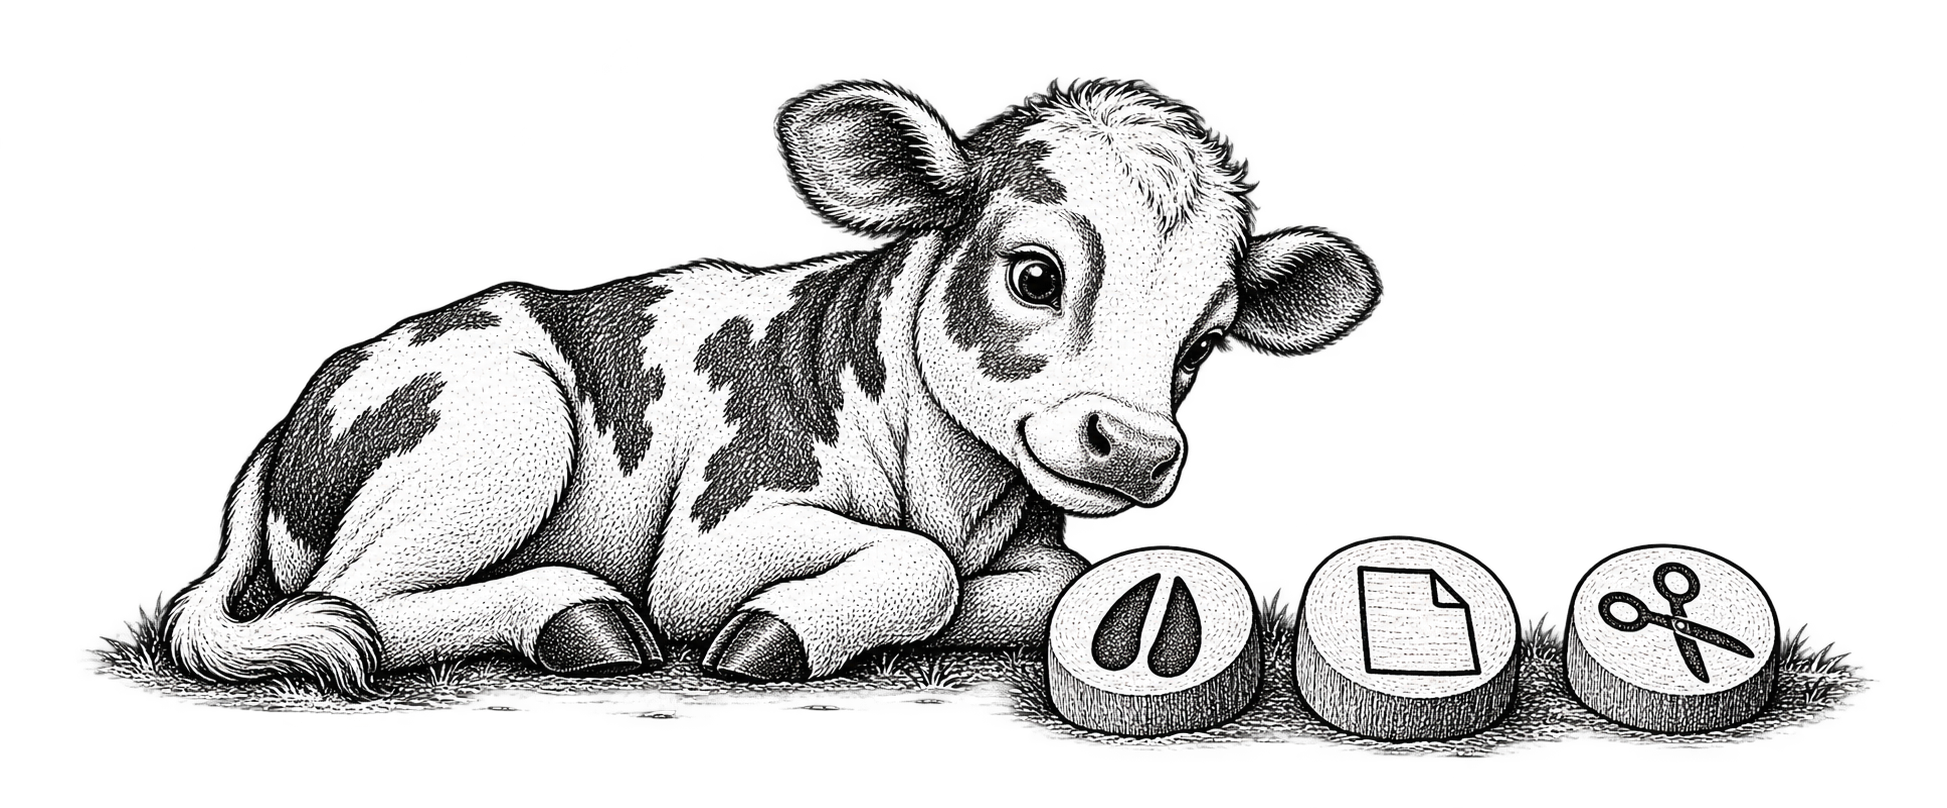
\includegraphics[width=174mm,height=94mm,keepaspectratio]{assets/cover.png}};
\node[anchor=north west,inner sep=0,text width=174mm] at ([xshift=18mm,yshift=-224mm]current page.north west)
{\fontsize{12}{16}\selectfont Understand what each step establishes\\and why it leads to the next.};
\node[anchor=west,inner sep=0] at ([xshift=18mm,yshift=-269mm]current page.north west)
{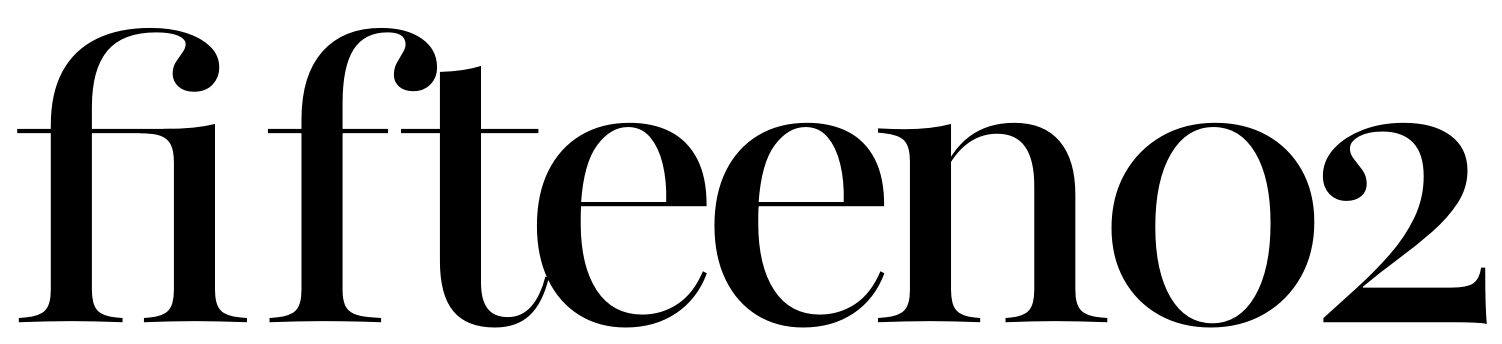
\includegraphics[width=43mm]{assets/logo.png}};
\node[anchor=east,inner sep=0] at ([xshift=192mm,yshift=-269mm]current page.north west)
{
\includegraphics[width=62mm]{assets/julians-pathfinder-monochrome.pdf}};
\node[anchor=north west,inner sep=0,text width=174mm] at ([xshift=18mm,yshift=-244mm]current page.north west) {\fontsize{11}{14}\selectfont \href{https://colab.research.google.com/github/fifteen02/julians-pathfinder/blob/main/Lesson\%205/lesson.ipynb}{\underline{Open this lesson in Google Colab}}};
\end{tikzpicture}\clearpage
\markboth{Questions}{}\raggedbottom\setlength{\parskip}{4pt}
{\heavy\fontsize{16}{20}\selectfont Lesson 5 / Hoof, Paper, Scissors\par}\medskip
\par\noindent\begin{minipage}{\linewidth}
{\heavy\fontsize{12}{15}\selectfont Plan gestures and count switches\par}\medskip
\textbf{L5-01 / Which gesture wins?}\par\smallskip H means hoof, P paper and S scissors. H beats S, S beats P, and P beats H. A win scores 1; a draw or loss scores 0. John plays H, H, S, S, P. Fill Bessie's wins in each round when she keeps H throughout, then when she keeps P or S.\par
\par\medskip \begingroup\small\setlength{\tabcolsep}{4pt}\renewcommand{\arraystretch}{1.35}\begin{tabularx}{\linewidth}{>{\raggedright\arraybackslash}X>{\raggedright\arraybackslash}X>{\raggedright\arraybackslash}X>{\raggedright\arraybackslash}X>{\raggedright\arraybackslash}X>{\raggedright\arraybackslash}X}\toprule\textbf{Round} & \textbf{0} & \textbf{1} & \textbf{2} & \textbf{3} & \textbf{4}\\\midrule
John & H & H & S & S & P\\
Keep H & ? & ? & ? & ? & ?\\
Keep P & ? & ? & ? & ? & ?\\
Keep S & ? & ? & ? & ? & ?\\
\bottomrule\end{tabularx}\endgroup\par\medskip 
\end{minipage}\par\vspace{4mm}
\par\noindent\begin{minipage}{\linewidth}
\textbf{L5-02 / Zero switches is already a useful case}\par\smallskip With no switches allowed, how would you solve the whole game? What answer do you get for H, H, S, S, P?\par
\end{minipage}\par\vspace{4mm}
\par\noindent\begin{minipage}{\linewidth}
\textbf{L5-03 / One well-placed switch}\par\smallskip John plays H, H, S, S, P. Bessie may choose her first gesture freely and change it at most once between rounds. Find a strategy with four wins. Number rounds from 0 and identify the gap where she changes. Can one change produce five wins?\par
\par\medskip \begingroup\small\setlength{\tabcolsep}{4pt}\renewcommand{\arraystretch}{1.35}\begin{tabularx}{\linewidth}{>{\raggedright\arraybackslash}X>{\raggedright\arraybackslash}X>{\raggedright\arraybackslash}X>{\raggedright\arraybackslash}X>{\raggedright\arraybackslash}X>{\raggedright\arraybackslash}X}\toprule\textbf{Round} & \textbf{0} & \textbf{1} & \textbf{2} & \textbf{3} & \textbf{4}\\\midrule
John & H & H & S & S & P\\
Bessie & ? & ? & ? & ? & ?\\
Wins & ? & ? & ? & ? & ?\\
\bottomrule\end{tabularx}\endgroup\par\medskip 
\end{minipage}\par\vspace{4mm}
\par\noindent\begin{minipage}{\linewidth}
\textbf{L5-04 / What must the state remember?}\par\smallskip Two strategies have processed the same rounds and used one switch, but one ends with H and the other with P. Can their best win counts be merged into one number?\par
\end{minipage}\par\vspace{4mm}
\par\noindent\begin{minipage}{\linewidth}
{\heavy\fontsize{12}{15}\selectfont Store scores and compare continuations\par}\medskip
\textbf{L5-05 / Recursive choices with a budget}\par\smallskip Write hps\_cached(john, budget) using recursion. Its helper knows the next round, switches left and previous gesture. How do you handle the first round without charging a switch?\par
\par\smallskip{\small\textbf{Start with:}}\par\smallskip\noindent\colorbox{codepaper}{\parbox{\dimexpr\linewidth-2\fboxsep\relax}{\small\ttfamily\raggedright def hps\_cached(john, budget):\\\hspace*{2.4em}def best(i, left, previous):\\\hspace*{4.8em}return None  \# Your helper goes here.\\\hspace*{2.4em}return best(0, budget, '')}}\par
{\small\textbf{What each function returns.}\par hps\_cached(john, budget): the most rounds Bessie can win within the switch budget.\par best(i, left, previous): the most further wins from round i, with left switches available and previous as the last gesture.\par }
{\small\textbf{Hints.}}\begin{itemize}\item What does best return when no rounds remain?\item When does choosing a gesture cost a switch, and when is it free?\item Which choices are not allowed with the switches left?\end{itemize}
\end{minipage}\par\vspace{4mm}
\par\noindent\begin{minipage}{\linewidth}
\textbf{L5-06 / Exactly used versus at most allowed}\par\smallskip John plays H in round 0. Fill Bessie's scores for each ending gesture H, P and S with exactly zero switches used. Can exactly one switch have been used after just this round? Write a dash for impossible states and explain why a score of 0 would mean something different.\par
\par\medskip \begingroup\small\setlength{\tabcolsep}{4pt}\renewcommand{\arraystretch}{1.35}\begin{tabularx}{\linewidth}{>{\raggedright\arraybackslash}X>{\raggedright\arraybackslash}X>{\raggedright\arraybackslash}X>{\raggedright\arraybackslash}X}\toprule\textbf{Switches used} & \textbf{End H} & \textbf{End P} & \textbf{End S}\\\midrule
0 & ? & ? & ?\\
1 & ? & ? & ?\\
\bottomrule\end{tabularx}\endgroup\par\medskip 
\end{minipage}\par\vspace{4mm}
\par\noindent\begin{minipage}{\linewidth}
\textbf{L5-07 / Stay or switch before this round}\par\smallskip After John plays H,H, scores for ending H,P,S are [0,2,0] with no switches and [1,1,1] with exactly one. John now plays S. For an ending H with exactly one switch, compare staying with H against changing from P or S. Then fill both new score rows.\par
\par\medskip \begingroup\small\setlength{\tabcolsep}{4pt}\renewcommand{\arraystretch}{1.35}\begin{tabularx}{\linewidth}{>{\raggedright\arraybackslash}X>{\raggedright\arraybackslash}X>{\raggedright\arraybackslash}X>{\raggedright\arraybackslash}X}\toprule\textbf{After H,H,S} & \textbf{End H} & \textbf{End P} & \textbf{End S}\\\midrule
0 switches & ? & ? & ?\\
1 switch & ? & ? & ?\\
\bottomrule\end{tabularx}\endgroup\par\medskip 
\end{minipage}\par\vspace{4mm}
\par\noindent\begin{minipage}{\linewidth}
\textbf{L5-08 / Trace all five rounds}\par\smallskip Trace John's rounds H,H,S,S,P. In each table column, 0 or 1 is the exact number of switches used; H, P or S is Bessie's ending gesture. Fill every row from the row immediately above it. A dash means impossible. Which final entry gives the best score with at most one switch?\par
\par\medskip \begingroup\small\setlength{\tabcolsep}{4pt}\renewcommand{\arraystretch}{1.35}\begin{tabularx}{\linewidth}{>{\raggedright\arraybackslash}l>{\raggedright\arraybackslash}X>{\raggedright\arraybackslash}X>{\raggedright\arraybackslash}X>{\raggedright\arraybackslash}X>{\raggedright\arraybackslash}X>{\raggedright\arraybackslash}X}\toprule\textbf{John prefix} & \textbf{0: H} & \textbf{0: P} & \textbf{0: S} & \textbf{1: H} & \textbf{1: P} & \textbf{1: S}\\\midrule
H & 0 & 1 & 0 & - & - & -\\
HH & ? & ? & ? & ? & ? & ?\\
HHS & ? & ? & ? & ? & ? & ?\\
HHSS & ? & ? & ? & ? & ? & ?\\
HHSSP & ? & ? & ? & ? & ? & ?\\
\bottomrule\end{tabularx}\endgroup\par\medskip 
\end{minipage}\par\vspace{4mm}
\par\noindent\begin{minipage}{\linewidth}
\textbf{L5-09 / Keep just the previous round}\par\smallskip Write hps\_table(john, budget) using a loop over rounds. Here used counts switches already used and g is the ending gesture. before[used][g] stores the best score after the previous round; now[used][g] includes the current round. Compare staying and switching. Why must now be fresh? Return the best score using at most budget switches (K in the original statement).\par
\par\smallskip{\small\textbf{Start with:}}\par\smallskip\noindent\colorbox{codepaper}{\parbox{\dimexpr\linewidth-2\fboxsep\relax}{\small\ttfamily\raggedright def hps\_table(john, budget):\\\hspace*{2.4em}return None  \# Replace with your answer.}}\par
{\small\textbf{What each function returns.}\par hps\_table(john, budget): the most rounds Bessie can win within the switch budget.\par }
{\small\textbf{Hints.}}\begin{itemize}\item What are the scores after round 0, and which states are impossible then?\item For a new cell, which cells of before lead to it by staying, and which by switching?\item What should an impossible state hold so that max ignores it?\end{itemize}
\end{minipage}\par\vspace{4mm}
\par\noindent\begin{minipage}{\linewidth}
{\heavy\fontsize{12}{15}\selectfont Test the budget and explain the state\par}\medskip
\textbf{L5-10 / Your turn: three different budgets}\par\smallskip Test your hps\_table(john, budget) from L5-09. For John = H,P,S, predict the best win count with budgets 0, 1 and 2. Give one strategy for each budget, then run your function.\par
\end{minipage}\par\vspace{4mm}
\par\noindent\begin{minipage}{\linewidth}
\textbf{L5-11 / More switches need not help}\par\smallskip Test your hps\_table(john, budget) from L5-09 on John = H,H,H with budgets 0 and 2, and on one round against S with budget 0. Predict each answer before running it. What should happen when the budget exceeds the useful number of changes?\par
\end{minipage}\par\vspace{4mm}
\par\noindent\begin{minipage}{\linewidth}
\textbf{L5-12 / The state is the explanation}\par\smallskip Choose a cell from the five-round score table and explain its round, exact switch count, ending gesture and stored score. Why can we forget the earlier gesture sequence once these facts and its best score are known? Compare this with Tower or Array Description.\par
\par\medskip \begingroup\small\setlength{\tabcolsep}{4pt}\renewcommand{\arraystretch}{1.35}\begin{tabularx}{\linewidth}{>{\raggedright\arraybackslash}X>{\raggedright\arraybackslash}X>{\raggedright\arraybackslash}X>{\raggedright\arraybackslash}X}\toprule\textbf{John prefix} & \textbf{Switches used} & \textbf{Ending gesture} & \textbf{Stored score}\\\midrule
 &  &  & \\
\bottomrule\end{tabularx}\endgroup\par\medskip 
\end{minipage}\par\vspace{4mm}
\end{document}